\documentclass{beamer}
\usepackage{tikz}
\usepackage{pgfplots}
%specify a certain package version to use
\pgfplotsset{compat=1.18}

\begin{document}
\begin{frame}{Example 1 - basic coordinate surface plot}
  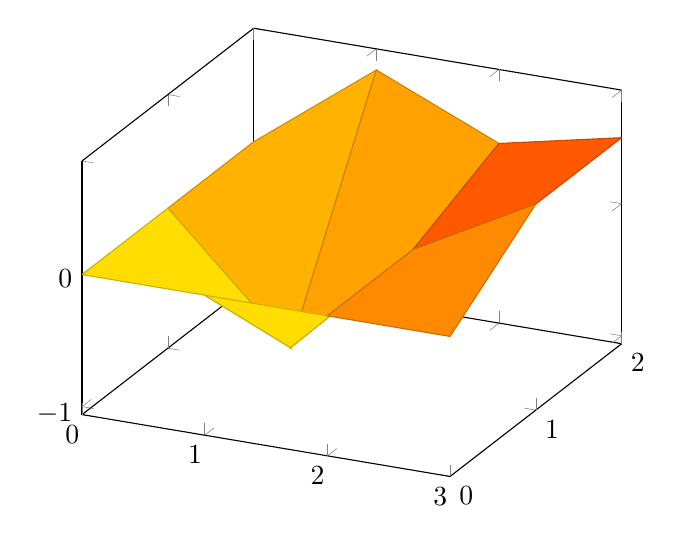
\begin{tikzpicture}
    \begin{axis}
      %From the PGFPlots manual.
      \addplot3 [surf] coordinates {
        (0,0,0) (1,0,0)   (2,0,0)   (3,0,0)
        
        (0,1,0) (1,1,-0.9) (2,1,0.0) (3,1,0.5)
 
        (0,2,0) (1,2,0.7) (2,2,0.3) (3,2,0.5)
      };
    \end{axis} 
  \end{tikzpicture}
\end{frame}

\begin{frame}{Example 2-basic, try using lualatex}
  %3D plots might be slow in the pasic pdflatex engine.
  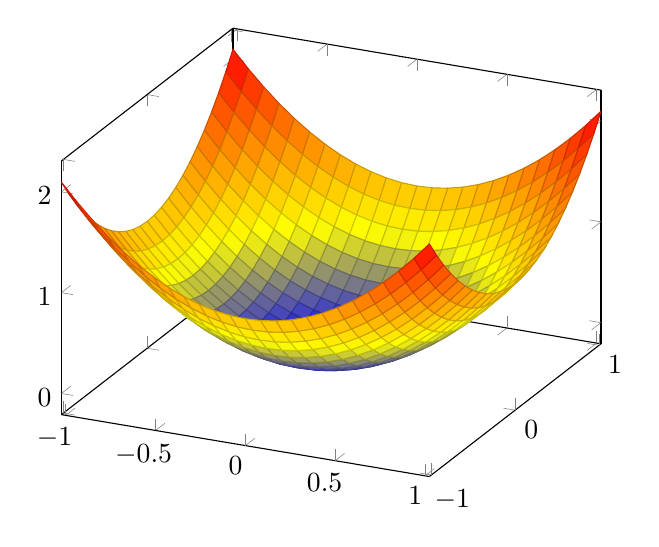
\begin{tikzpicture}
    \begin{axis}
      \addplot3+ [domain=-1.024:1.024,surf,no marks] {x * x + y * y};
    \end{axis}
  \end{tikzpicture}
\end{frame}

\begin{frame}{Example 2-gnuplot, try using shell-escape}
  %Look up shell-escape or write18 to be able to run this. 
  \begin{tikzpicture}
    \begin{axis}
      \addplot3+ [domain=-1.024:1.024,surf,no marks]  gnuplot {x * x + y * y};
    \end{axis}
  \end{tikzpicture}
\end{frame}

\begin{frame}{Example 3, different colouring}
  %colormap/cool gives the blue colouring
  %shader=interp interpolates every pixel.
  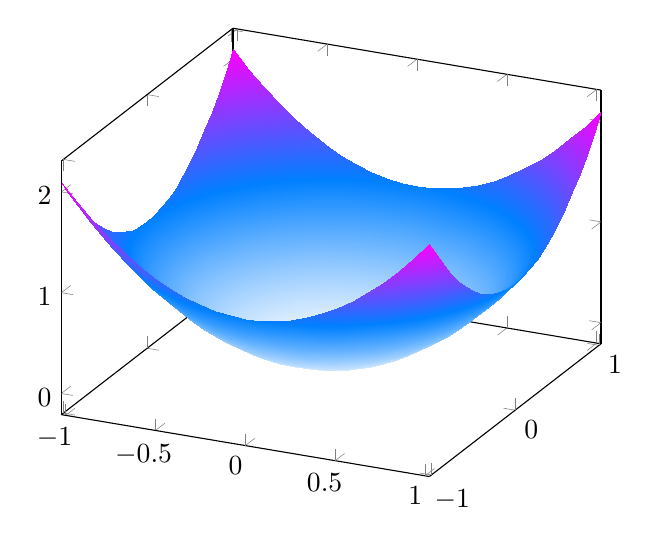
\begin{tikzpicture}
    \begin{axis}[colormap/cool]
      \addplot3+ [domain=-1.024:1.024,surf,no marks,shader=interp] {x * x + y * y};
    \end{axis}
  \end{tikzpicture}
\end{frame}

\begin{frame}{Example 4, contour gnuplot and projection}
  %A contour gnuplot is a 3D contour plot which requires gnuplot to compute it.
  \begin{tikzpicture}
    \begin{axis}[colormap/cool]
      \addplot3+ [
        domain=-1.024:1.024,
        no marks,
        contour gnuplot={
          number=20, %how many contours
	  labels=false
        }
      ]
       {x * x + y * y};
      \addplot3+ [
        domain=-1.024:1.024,
        no marks,
        contour gnuplot={
          number=20,
	  labels=false,
          %otherwise the z filter will not work:
          %give each point metadata its raw z value,
          %so we can filter it below
          output point meta=rawz,
        },
        %force the z-value to a constant, so we can project the plot.
        z filter/.code={\def\pgfmathresult{-1}} 
      ]
                 {x * x + y * y};

    \end{axis}
  \end{tikzpicture}
\end{frame}

\begin{frame}{Example 5, plot and projection}
  \begin{tikzpicture}
    \begin{axis}[colormap/cool]
      \addplot3+ [
        domain=-1.024:1.024,
        no marks,
        contour gnuplot={
          number=20,
	  labels=false,
          output point meta=rawz,
        },
        z filter/.code={\def\pgfmathresult{-1}}
      ]
                 {x * x + y * y};

      \addplot3+ [
        domain=-1.024:1.024,
        no marks,
        surf
      ]
      gnuplot {x * x + y * y};
    \end{axis}
  \end{tikzpicture}
\end{frame}




\begin{frame}{Example 6}
  \begin{tikzpicture}
    \begin{axis} [
        title={Subspecies separation},
        xlabel=Sepal length,
        ylabel=Sepal width,
        zlabel=Petal length,
        %legend, %would get in the way at default settings
        legend style ={anchor=north west, align=left},
        view={-30}{30},%rotate the axis
      ]
      \addplot3[only marks, mark=o,draw=red] table[col sep=comma,x=sepal_length,y=sepal_width,z=petal_length]{iris.csv};
      \addlegendentry{Everything};
    \end{axis} 
  \end{tikzpicture}
\end{frame}




\begin{frame}{Task 1: Rastrigin's function - like this}
  \centering
  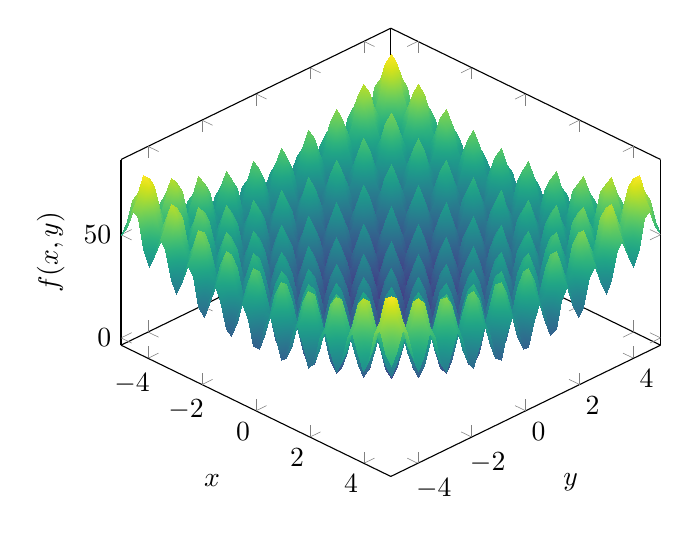
\begin{tikzpicture}
    \begin{axis}[
      colormap/viridis, 
      view={45}{45},
      samples=50,
      domain=-5:5,
      xlabel={$x$}, ylabel={$y$}, zlabel={$f(x,y)$}
    ]
      \addplot3[surf, shader=interp] 
      {20 + x^2 + y^2 - 10*(cos(deg(2*pi*x)) + cos(deg(2*pi*y)))};
    \end{axis}
  \end{tikzpicture}
\end{frame}

\begin{frame}{Task 2: 3D scatterplot}
  \centering
  \begin{tikzpicture}
    \begin{axis} [
        title={Subspecies separation},
        xlabel=Sepal length, ylabel=Sepal width, zlabel=Petal length,
        view={-30}{30},
        legend pos=outer north east,
        scatter/classes={
          setosa={mark=o, blue},
          versicolor={mark=triangle, red},
          virginica={mark=diamond, black}
        }
      ]
      
      \addplot3[
          only marks, 
          scatter, 
          scatter src=explicit symbolic,
          mark size=2pt
      ] table[
          col sep=comma, 
          x=sepal_length, 
          y=sepal_width, 
          z=petal_length, 
          meta=species 
      ]{iris.csv};
      
      \addplot3[
          surf, 
          opacity=0.1, 
          samples=2, 
          domain=4:7, 
          y domain=2:4.5, 
          blue!20, 
          shader=flat
      ] {2};
      \node at (axis cs:4.5,4,2.2) [blue, font=\tiny] {Setosa Boundary};
      
      \legend{Setosa, Versicolor, Virginica}
    \end{axis} 
  \end{tikzpicture}
\end{frame}




\end{document}
